\chapter{Discussão}
\label{cap:discussao}
\phantom{0}

Este capítulo apresentada vários estudos de caso, bem como uma comparação do método proposto com os trabalhos relacionados encontrados na literatura (Capítulo~\ref{cap:trabalhos-relacionados}). Por fim, são discutidas as vantagens e limitações do método.

\section{Estudos de Caso – Segmentação de Rins}
\label{sec:estudos-segmentacao-rins}

Esta seção apresenta um conjunto de estudos de caso para analisar a influência das etapas propostas na segmentação de rins. Os casos observados foram: (1) a segmentação inicial apresentou uma segmentação precisa e as demais etapas não foram necessárias; (2) as etapas de reconstrução dos tumores renais e pós-processamento reduziram ligeiramente o desempenho da segmentação inicial; e (3) as etapas de reconstrução de tumores renais e pós-processamento foram necessárias e capazes de melhorar a qualidade da segmentação inicial.

\subsection{Estudo de Caso 1 – Paciente case\_00018}
\label{sec:estudo-rins-1}

O primeiro estudo de caso trata de um exame em que as etapas de reconstrução e pós-processamento dos tumores foram desnecessárias. Este caso é ilustrado na Figura~\ref{fig:estudo-rins-1}, onde pode-se ver que nenhum fragmento segmentado está presente, exceto os rins. Além disso, é notável que a etapa de reconstrução dos tumores renais (Figura~\ref{fig:estudo-rins-1}~(c), em cinza a segmentação inicial dos rins e em verde a reconstrução dos tumores renais) não contribuiu para uma maior segmentação na região renal, uma vez que as regiões reconstruídas dos tumores renais já haviam sido segmentadas na etapa inicial (dentro do rim). A segmentação dos rins obteve 94,67\% Dice, 89,88\% Jaccard, 99,91\% de acurácia, 99,88\% de sensibilidade e 99,91\% de especificidade. Após as etapas de reconstrução e pós-processamento (Figura~\ref{fig:estudo-rins-1} (d)) dos tumores, os resultados permaneceram os mesmos. Portanto, a segmentação inicial foi capaz de determinar contornos renais muito precisos. Esse tipo de comportamento foi encontrado em 4 pacientes.

\begin{figure}[!ht]
    \centering
    \caption{Estudo de caso 1. Segmentações dos rins (cinza) e reconstrução dos tumores renais (verde).}
    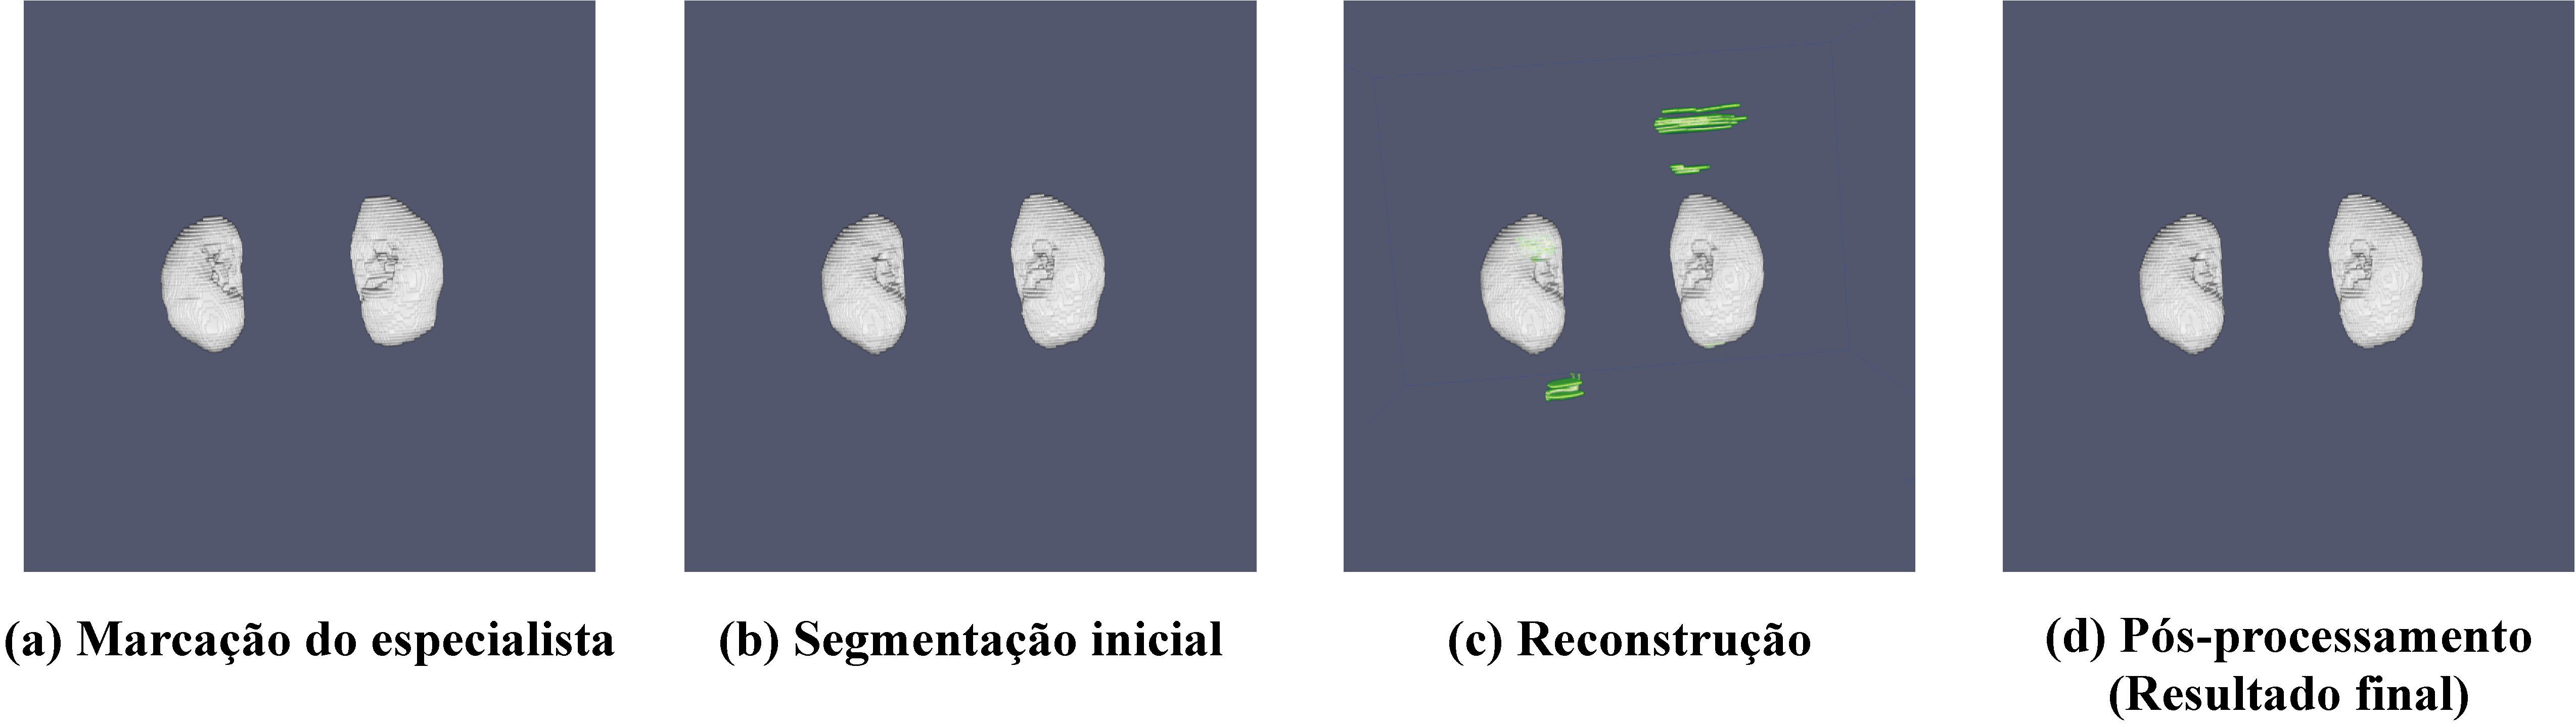
\includegraphics[width=1\textwidth]{figuras/estudos-casos-rins-1-18.pdf}
    \label{fig:estudo-rins-1}
    \legend{Fonte: Elaborado pela autora.}
\end{figure}

\subsection{Estudo de Caso 2 – Paciente case\_00149}
\label{sec:estudo-rins-caso-2}

Neste estudo de caso, as etapas de reconstrução e pós-processamento dos tumores afetaram sutilmente a segmentação inicial. Pode-se ver na Figura~\ref{fig:estudo-rins-2} que a combinação das etapas descritas não foi capaz de melhorar os resultados da segmentação inicial. A etapa mais crítica foi a reconstrução de tumores renais (Figura~\ref{fig:estudo-rins-2} (c)), na qual é possível observar que comprometeu a região renal com mais fragmentos de falsos positivos. A segmentação inicial obteve 98,48\% Dice, 97,00\% Jaccard, 99,95\% de acurácia, 98,37\% de sensibilidade e 99,98\% de especificidade e a segmentação final (reconstrução + pós-processamento) obteve 98,37\% Dice, 96,79\% Jaccard, 99,94\% de acurácia, 98,50\% de sensibilidade e 99,97\% de especificidade. Apesar disso, as taxas de desempenho da maioria dos quantificadores não foram tão afetadas. Esse tipo de comportamento foi encontrado em apenas 2 pacientes.

\begin{figure}[!ht]
    \centering
    \caption{Estudo de caso 2. Segmentações dos rins (cinza) e reconstrução dos tumores renais (verde).}
    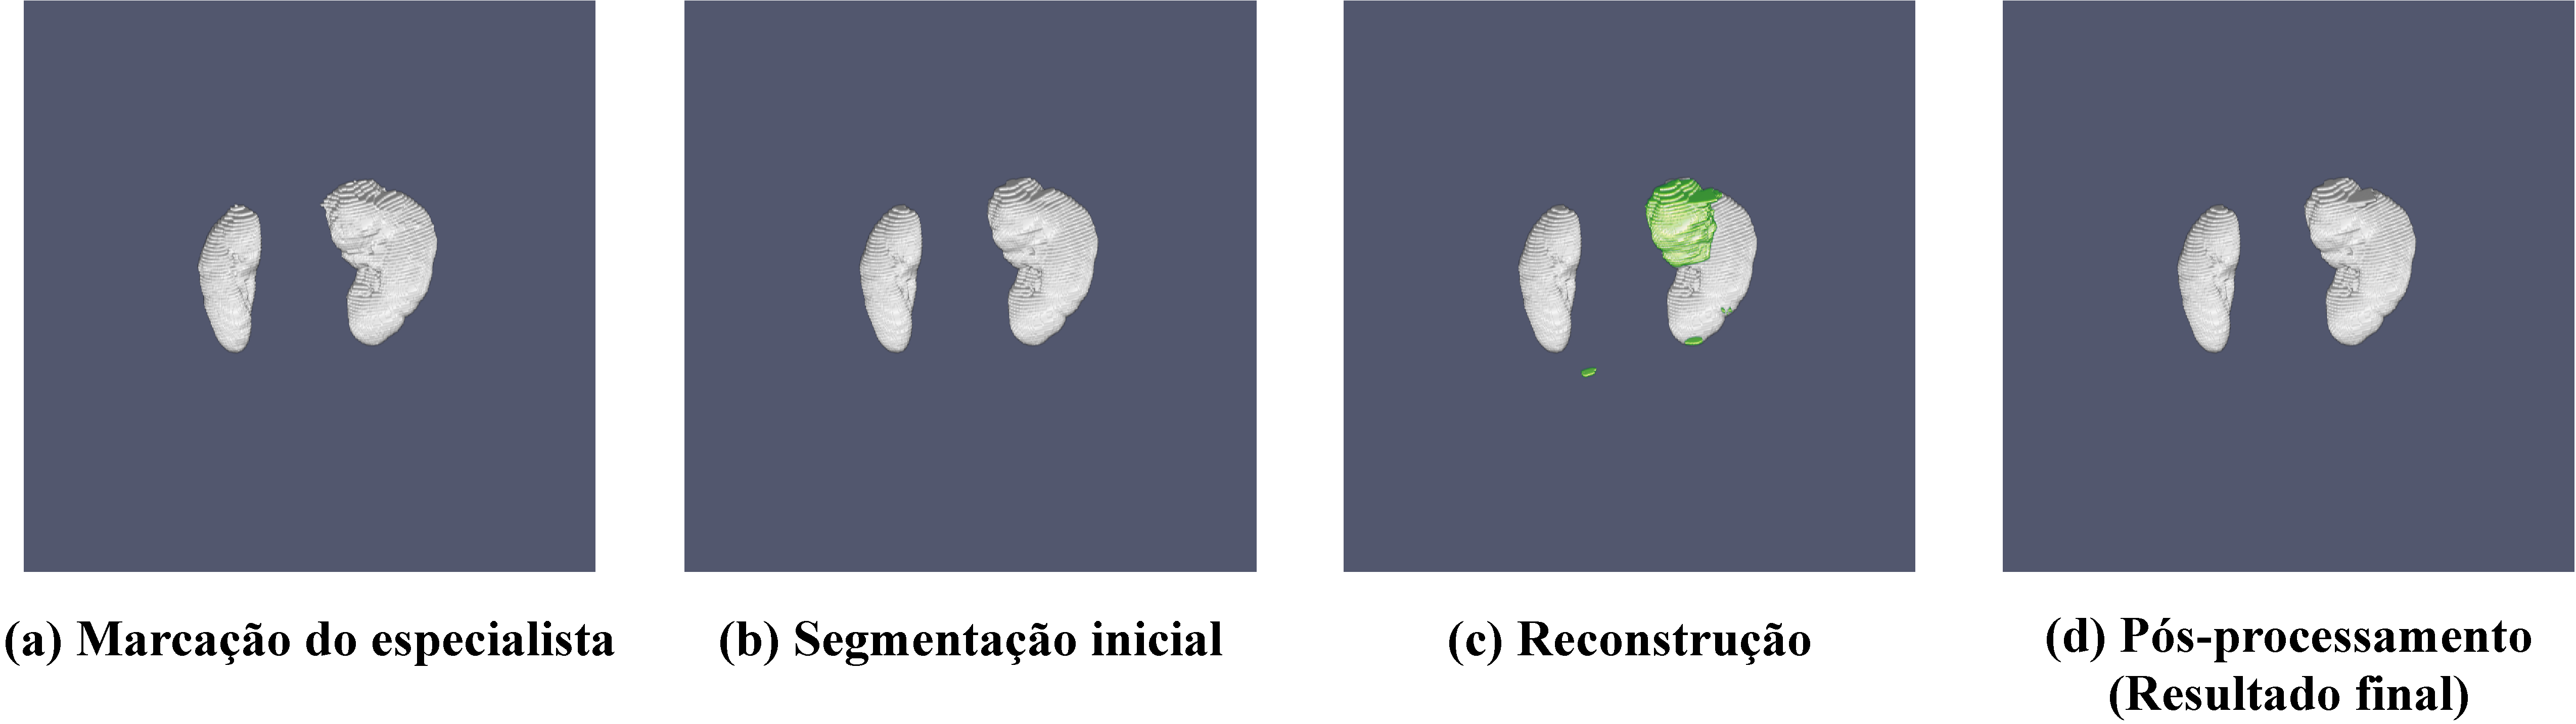
\includegraphics[width=1\textwidth]{figuras/estudos-casos-rins-2-149.pdf}
    \label{fig:estudo-rins-2}
    \legend{Fonte: Elaborado pela autora.}
\end{figure}

\subsection{Estudo de Caso 3 – Paciente case\_00045}
\label{sec:estudo-rins-caso-3}

No último estudo de caso dos rins, as etapas de reconstrução e pós-processamento dos tumores funcionaram bem. É possível ver na Figura~\ref{fig:estudo-rins-3} que a segmentação inicial dos rins gerou alguns fragmentos errôneos (falsos positivos). Além disso, algumas regiões renais não foram segmentadas, porém a reconstrução dos tumores renais foi capaz de suprir essa deficiência, pois conseguiu recuperar regiões tumorais que consequentemente também fazem parte dos rins (Figura~\ref{fig:estudo-rins-3} (c)). Finalmente, com a aplicação do pós-processamento (Figura~\ref{fig:estudo-rins-3} (d)), pode-se ver como a marcação do método proposto é muito semelhante à marcação do especialista. Nesse caso, a segmentação inicial atingiu 89,93\% de Dice, 81,71\% de Jaccard, 99,81\% de acurácia, 86,63\% de sensibilidade e 99,94\% de especificidade. Após as etapas de reconstrução e pós-processamento dos tumores, os resultados foram 94,78\% Dice, 90,07\% Jaccard, 99,89\% de acurácia, 96,31\% de sensibilidade e 99,92\% de especificidade, basicamente uma melhoria de 4,85\% de Dice em relação à segmentação inicial. Foram encontrados 25 pacientes semelhantes a este comportamento.

\begin{figure}[!ht]
    \centering
    \caption{Estudo de caso 3. Segmentação dos rins (cinza) e reconstrução dos tumores renais (verde).}
    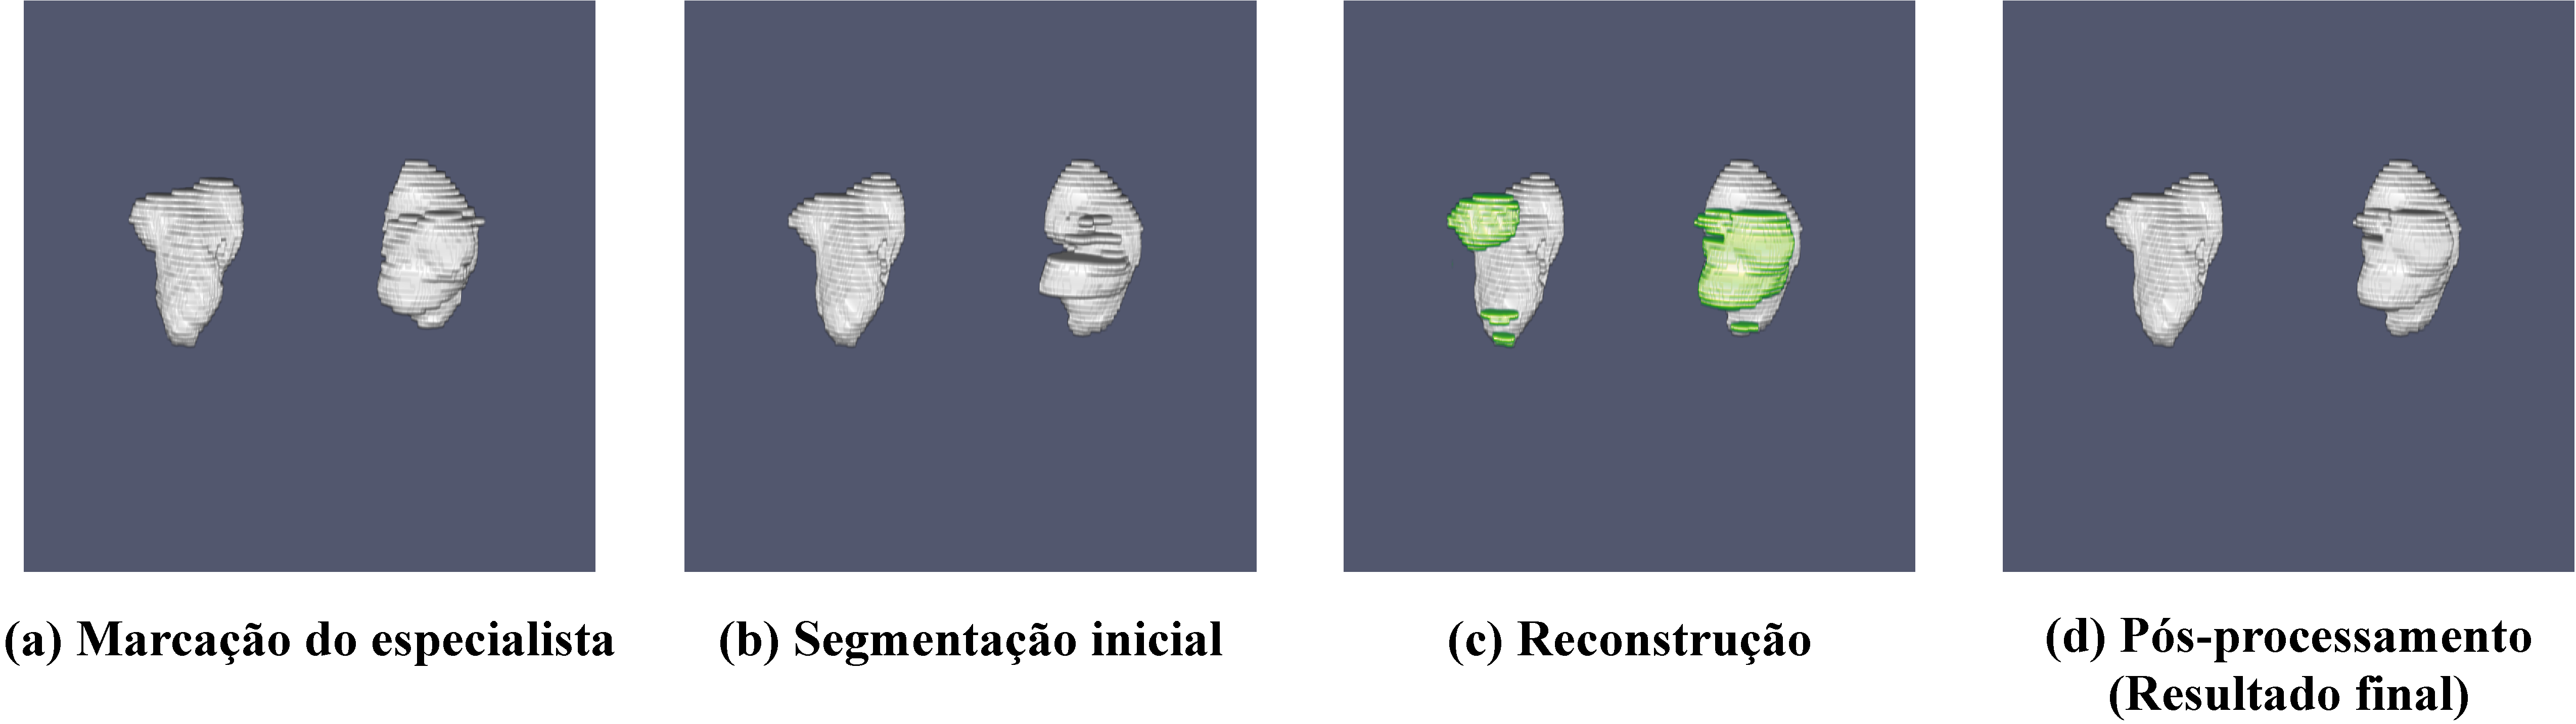
\includegraphics[width=1\textwidth]{figuras/estudos-casos-rins-3-45.pdf}
    \label{fig:estudo-rins-3}
    \legend{Fonte: Elaborado pela autora.}
\end{figure}

\section{Estudos de Caso – Segmentação de Tumores Renais}
\label{sec:estudos-segmentacao-tumores-renais}

Nesta seção, são mostradas e discutidas as situações mais comuns observadas na aplicação das etapas do método proposto para a segmentação de tumores. Os cenários encontrados foram os seguintes: (1) as etapas de reconstrução de tumores renais e pós-processamento afetaram a qualidade da segmentação inicial dos candidatos a tumores renais na região renal; e (2) as etapas de reconstrução de tumores renais e pós-processamento melhoraram a segmentação inicial dos candidatos a tumores renais na região renal.

\subsection{Estudo de Caso 1 – Paciente case\_00012}
\label{sec:estudo-tumores-caso-1}

O primeiro estudo de caso explora uma circunstância em que as etapas de reconstrução e pós-processamento dos tumores afetaram a segmentação inicial de candidatos a tumores renais na região renal. Observa-se na Figura~\ref{fig:estudo-tumores-1} a entrada da rede de segmentação (segmentação final dos rins), a marcação do especialista (b) e as etapas do método proposto (c) e (d). Após as duas últimas etapas (Figura~\ref{fig:estudo-tumores-1} (d)), houve uma deterioração no desempenho em comparação com a segmentação inicial. Neste caso, os resultados finais foram 89,85\% de Dice, 81,57\% de Jaccard, 99,92\% de acurácia 98,71\% de sensibilidade e 99,92\% especificidade. No entanto, a segmentação inicial atingiu 90,69\%, 82,97\%, 99,92\%, 98,04\% e 99,93\% de Dice, Jaccard, acurácia, sensibilidade e especificidade, respectivamente. Dessa forma, as etapas de reconstrução e pós-processamento dos tumores não foram capazes de definir com maior precisão as regiões dos tumores. Este cenário foi observado em 4 pacientes.

%Apesar disso, as taxas de desempenho para a maioria das métricas não mudaram significativamente.

\begin{figure}[!ht]
    \centering
    \caption{Estudo de caso 1. Segmentação dos rins (cinza), segmentação dos tumores renais (vermelho) e reconstrução dos tumores renais (verde).}
    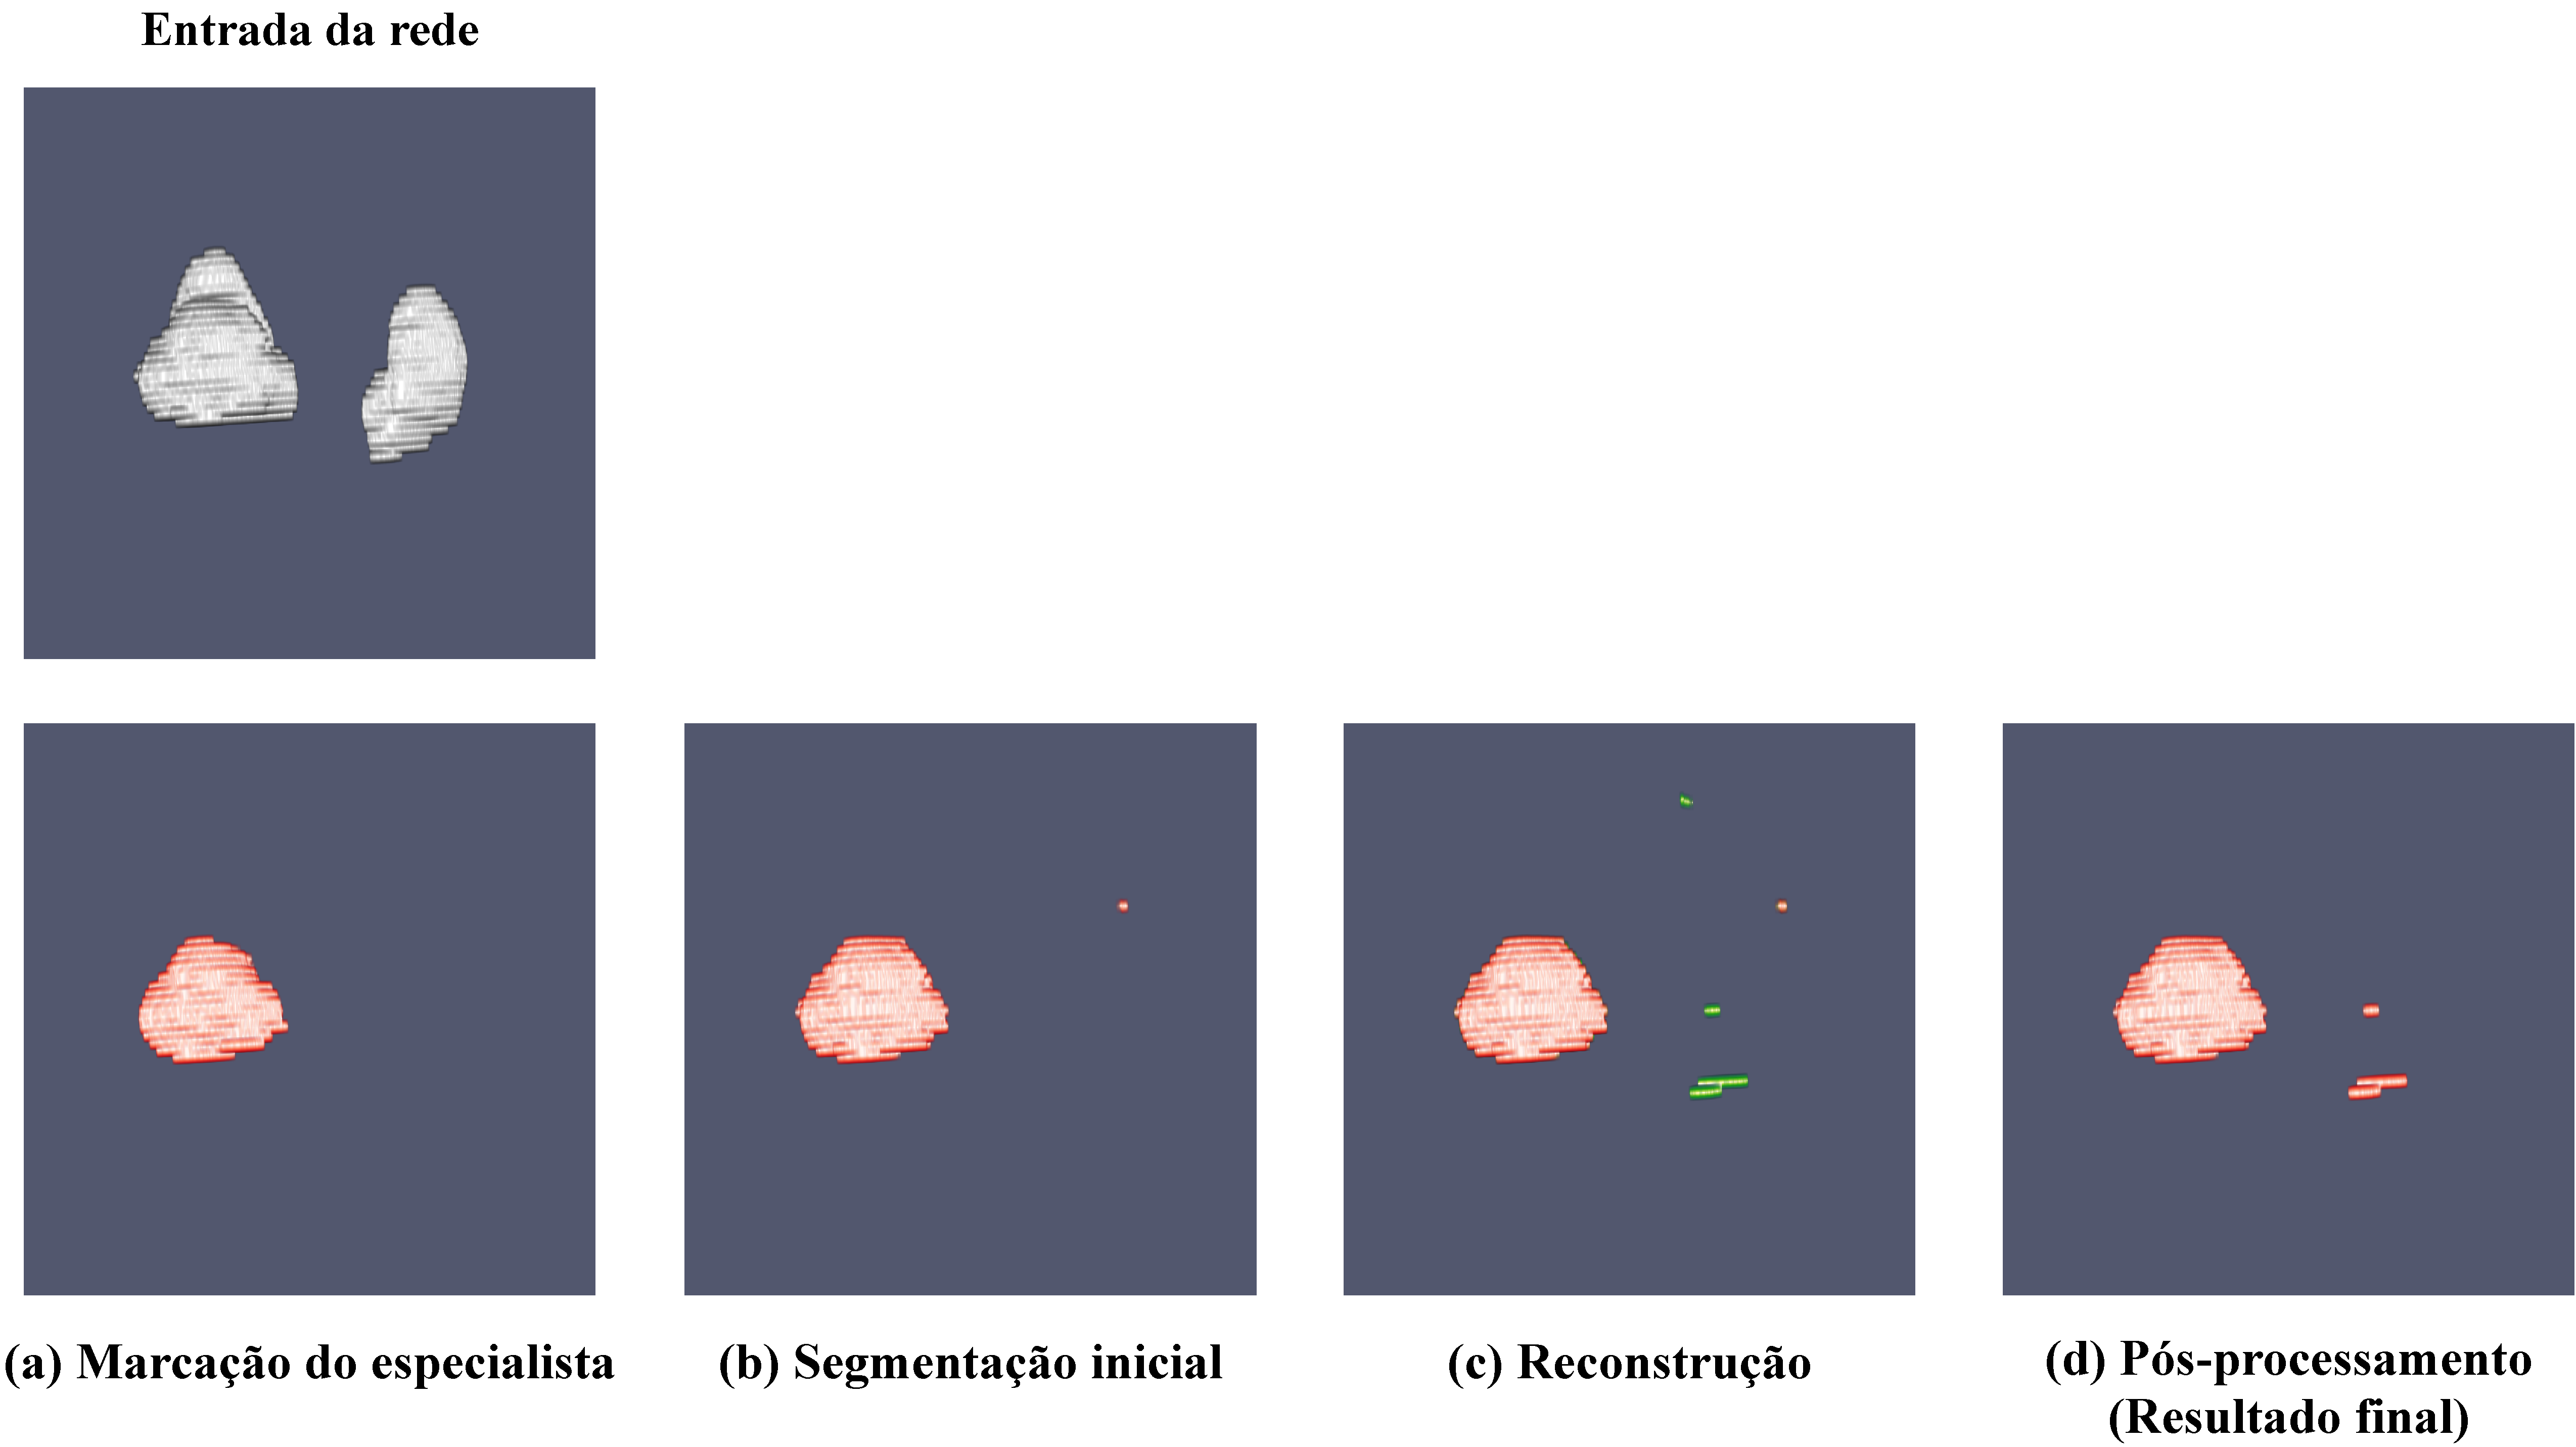
\includegraphics[width=1\textwidth]{figuras/estudos-casos-tumores-renais-1-12.pdf}
    \label{fig:estudo-tumores-1}
    \legend{Fonte: Elaborado pela autora.}
\end{figure}

\subsection{Estudo de Caso 2 – Paciente case\_00028}
\label{sec:estudo-tumores-caso-2}

Neste estudo de caso, as etapas de reconstrução e pós-processamento dos tumores compensaram algumas deficiências da segmentação inicial. Na Figura~\ref{fig:estudo-tumores-2} (b), observa-se que a segmentação inicial gerou vários fragmentos errôneos. Porém, após as etapas de reconstrução e pós-processamento (Figura~\ref{fig:estudo-tumores-2} (c) e Figura~\ref{fig:estudo-tumores-2} (d), respectivamente), a segmentação pelo método proposto eliminou um grande número de falsos positivos. Neste caso, foram obtidos 94,50\% de Dice, 89,57\% Jaccard, 99,97\% de acurácia, 93,85\% de sensibilidade e 99,98\% de especificidade na segmentação final, basicamente uma melhoria significativa de 27,67\% na métrica Dice em comparação com a segmentação inicial, onde os resultados foram 66,83\% de Dice, 50,18\% de Jaccard, 99,84\% de acurácia, 51,52\% de sensibilidade e 99,99\% de especificidade. Este cenário foi observado em 27 casos de teste.

\begin{figure}[!ht]
    \centering
    \caption{Estudo de caso 2. Segmentação dos rins (cinza), segmentação dos tumores renais (vermelho) e reconstrução dos tumores renais (verde).}
    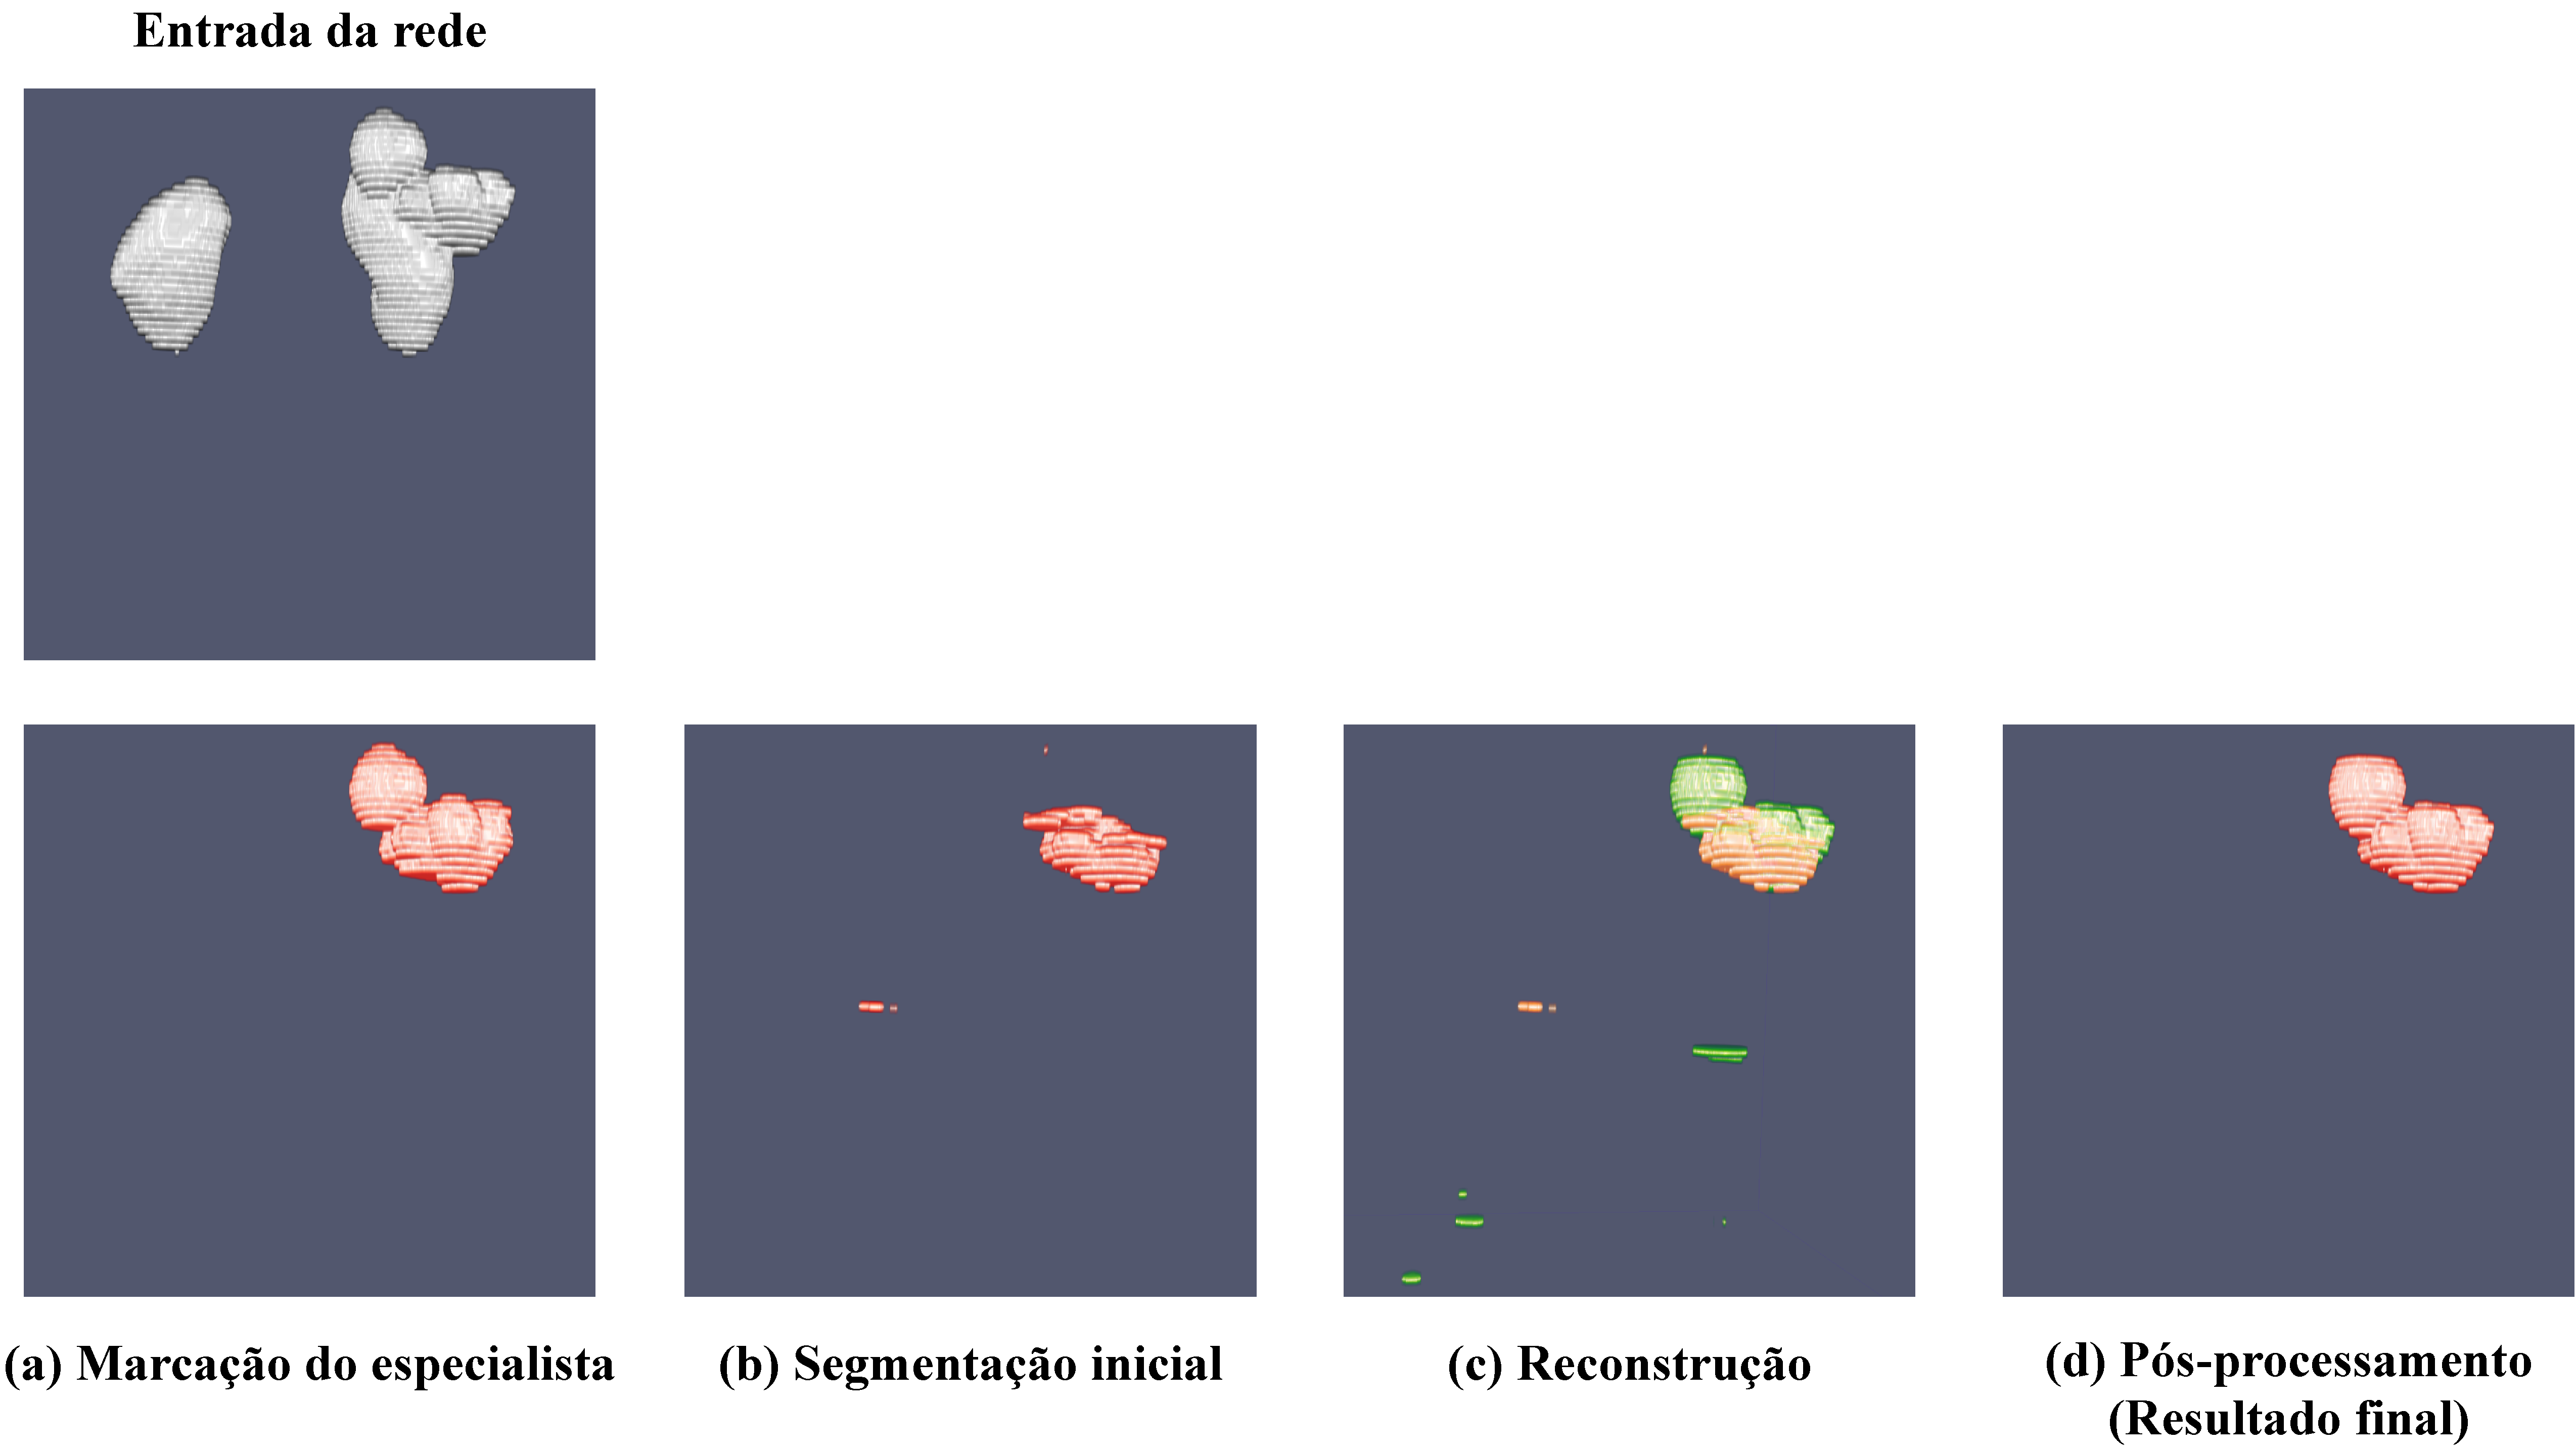
\includegraphics[width=1\textwidth]{figuras/estudos-casos-tumores-renais-2-28.pdf}
    \label{fig:estudo-tumores-2}
    \legend{Fonte: Elaborado pela autora.}
\end{figure}

%\subsection{Estudo de Caso 3 – Vários Pacientes}
%\label{sec:estudo-tumores-caso-3}

%Neste último cenário, pretende-se mostrar que o método proposto é eficiente mesmo quando não há tumores renais em um rim. Esse cenário é ilustrado na Figura~\ref{} na qual são mostrados vários pacientes que tem esse comportamento. Por meio da marcação do especialista (imagem superior) é possível observar que há tumores renais em apenas um rim. Na imagem central da Figura~\ref{}  é obtida a segmentação inicial dos rins (cinza) e candidatos a tumores renais na região renal (vermelho), na qual pode-se observar que os tumores renais foram segmentados apenas no rim que realmente possui tumores. Conforme ilustrado, percebe-se que após a aplicação das etapas de reconstrução dos tumores renais e pós-processamento (imagem inferior), o método proposto permanece consistente e continua melhorando os resultados dos rins e das regiões que apresentam tumores renais. Portanto, conclui-se que o método proposto funciona bem mesmo quando não há tumores renais nos rins. Isso prova que o método pode ser usado mesmo em cenários em que não há tumores renais para segmentar.

\section{Comparação do Método Proposto com os Trabalhos Relacionados}
\label{sec:comparacao}

Nesta seção é apresentada uma análise comparativa dos resultados obtidos pelo método proposto em relação aos trabalhos relacionados (Capítulo~\ref{cap:trabalhos-relacionados}). As subseções a seguir apresentam uma comparação com os trabalhos relacionados à segmentação de rins, segmentação de tumores, e segmentação de rins e tumores renais.

\subsection{Segmentação de Rins}
\label{sec:disc-trab-relac-rins}

Esta subseção mostra os resultados dos trabalhos relacionados à segmentação de rins. A Tabela~\ref{tab:res-trabalhos-relacionados-rins} apresenta um resumo desta comparação, fornecendo informações das técnicas, quantidade de pacientes e as métricas de desempenho usadas em seus métodos. Por fim, são apresentados os resultados do método proposto. 

\begin{table}[!ht]
\caption{Comparação dos resultados do método com trabalhos relacionados à segmentação de rins.}
\label{tab:res-trabalhos-relacionados-rins}
\centering
%\setstretch{1.3}
\doublespacing
\resizebox{\columnwidth}{!}{
\begin{tabular}{p{11cm}ccccccc}
\hline
\centering \textbf{Técnica(s)}                                                                                                       & \textbf{Base} & \textbf{Pacientes} & \textbf{Dice (\%)} & \textbf{Jacc (\%)} & \textbf{Acc (\%)} & \textbf{Sen (\%)} & \textbf{Esp (\%)} \\ \hline
Modelo deformável baseado em \textit{Level Set} \cite{khalifa2011new}                                                     & Privada       & 29                 & 95                 & -                  & 96,36             & 93,8              & -                 \\
Esquema hierárquico de registro e ponderação de atlas \cite{wolz2013automated}                                            & Privada       & 150                & 92,5               & 86,8               & -                 & 98,3              & -                 \\
Continuidade contextual na sequência de imagens de TC \cite{Zhao2013ContextualIK}                                         & Privada       & 10                 & 94,7               & -                  & -                 & -                 & -                 \\
Registro de imagens multi-atlas \cite{yang2014automatic}                                                                  & Privada       & 14 fatias          & 95,2               & -                  & -                 & -                 & -                 \\
Estrutura híbrida baseada de modelos geométricos deformáveis e NMF \cite{khalifa2016kidney}                               & Privada       & 36                 & 96,45              & -                  & -                 & -                 & -                 \\
Contorno ativo usando a estrutura \textit{Level Set} \cite{skalski2017kidney}                                             & Privada       & 10                 & 86,2               & -                  & -                 & -                 & -                 \\
CNNs 3D \cite{jackson2018deep}                                                                                            & Privada       & 113                & 88,5               & -                  & -                 & -                 & -                 \\
Crowdsourcing e CNN \cite{mehta2019segmenting}                                                                            & Privada       & 42                 & 93,2               & -                  & -                 & -                 & -                 \\
U-Net, \textit{patch} e sistema de rastreamento \cite{9534007}                                                            & KiTS19        & 270                & 90,63              & -                  & -                 & -                 & -                 \\ \hline
\textbf{Método proposto com ResUNet 2.5D, DeepLabv3+ 2.5D, agrupador de tumores e técnicas para remover falsos positivos} & KiTS19        & 210                & 97,45              & 95,05              & 99,95             & 98,44             & 99,96             \\ \hline
\end{tabular}
}
\end{table}

Nos últimos anos, muitas técnicas de segmentação renal foram desenvolvidas e aplicadas em diversos estudos. Por exemplo,  \citeonline{khalifa2011new} usaram modelos deformáveis baseados em conjuntos de níveis geométricos para segmentação renal em TC. \citeonline{khalifa2016kidney} também fizeram uso de modelos deformáveis. Os modelos deformáveis são controlados por informações sobre a intensidade e a forma estatística dos rins. Em casos de ruído, imagens de baixa resolução e limites difusos, pode aumentar a instabilidade quanto à identificação dos contornos renais e resultar em falhas no método. \citeonline{khalifa2011new} atingiram um Dice de 95\%, acurácia de 96,36\% e sensibilidade de 93,8\%, considerando apenas 29 pacientes. Em \citeonline{khalifa2016kidney} 95\% de Dice foram alcançados, considerando 36 pacientes. Os dois estudos fazem uso de TCs de pacientes saudáveis, ou seja, sem presença de tumores ou cistos. O método proposto nesta tese usa TCs de pacientes com presença de anormalidades, o que dificulta a segmentação dos rins. Ainda assim, este método superou os resultados dos dois trabalhos descritos.

Alguns trabalhos que usaram atlas e registros foram propostos por \citeonline{wolz2013automated} e \citeonline{yang2014automatic} alcançando métricas promissoras na tarefa de segmentação renal. A desvantagem de suas abordagens é que geralmente elas tem um certo tamanho para resolver o problema em um conjunto de imagens e, ao testar novas imagens de tamanhos diferentes do atlas, o método não tem garantia de funcionar. Observe que em \citeonline{wolz2013automated} o conjunto de imagens usado para validar o método contém 150 pacientes saudáveis e em \citeonline{yang2014automatic} apenas 14 fatias são usadas, das quais seis resultados de segmentação renal com grandes tumores foram excluídos porque o tumor alterou significativamente a forma do rim. O método aqui proposto não usa atlas e registros, o que o torna mais robusto na tarefa de segmentação renal. Além disso, todas as imagens de TC disponíveis na base de imagens foram utilizadas, independentemente dos resultados. O índice de Dice alcançado em nosso método proposto foi de 97,45\%.

O método proposto por \citeonline{Zhao2013ContextualIK} faz uso da continuidade contextual de fatias adjacentes em imagens de TC, então uma estrutura de segmentação baseada em fatias é construída para segmentar automaticamente os rins. Para este propósito, quatro parâmetros contextuais, incluindo distância e sobreposição, são selecionados para estimar a continuidade entre fatias adjacentes. Para isso, utilizam-se algoritmos convencionais de segmentação e modificação (modelo deformável tradicional e limiar iterativo local), chegando a 94,7\% de Dice, utilizando um banco de dados privado composto por 10 pacientes com doenças renais. No método em estudo, propõe-se o uso de duas redes neurais convolucionais para atingir uma segmentação precisa para os rins, assim, são inseridas abordagens capazes de segmentar sem a necessidade de um ponto de partida.

A segmentação dos rins baseada no método Contorno Ativo usando uma estrutura \textit{Level Set} com restrições elipsoidais foi proposta em \citeonline{skalski2017kidney}. A solução proposta leva em consideração as informações sobre a região e os termos de contorno, bem como as restrições dedicadas à característica de formato do rim, o que torna o método bastante restrito e, não é garantido que o método funcione bem com o surgimento de novas imagens com formatos ligeiramente diferentes. O método foi testado em 10 tomografias de pacientes com câncer renal, obtendo resultados de 86,2\% de Dice. Em nossa proposta não há necessidade de informações anatômicas, e alcançou resultados superiores a 97\% de Dice usando 31 pacientes com tumores. \citeonline{jackson2018deep} desenvolveram uma ferramenta automatizada com base em CNNs 3D e alcançaram 88,5\% de Dice usando 113 TCs e \textit{data augmentation offline}.

Em \citeonline{mehta2019segmenting}, os autores usaram uma rede neural convolucional e uma ferramenta de \textit{crowdsourcing} para segmentação de órgãos em larga escala. As validações foram realizadas comparando as segmentações de \textit{crowdsourcing} e segmentações marcadas por especialistas, e verificou que o desempenho não foi significativamente diferente. Porém, a realização de marcações renais por usuários sem o conhecimento especializado na área é imprudente, pois isso pode ser feita de forma errada e afetar a segmentação dos rins e, consequentemente, gerar resultados errados. Os resultados foram 93,2\% de Dice usando para validar uma base de 42 pacientes saudáveis. \citeonline{9534007} apresentaram um método composto por duas etapas. Na primeira etapa, é realizada a segmentação semântica baseada na rede U-Net e \textit{batch}. Na segunda etapa, um sistema de rastreamento (\textit{middle-bottom, middle-top}) foi usado para encontrar contornos do rim nas fatias de TC restantes. O método desenvolvido atingiu um Dice de 90,63\%.

\subsection{Segmentação de Tumores Renais}
\label{sec:disc-trab-relac-tumor-renal}

Esta segunda subseção apresentada uma análise comparativa do método proposto com os trabalhos relacionados à segmentação de tumores renais. O resumo desses trabalhos é apresentado na Tabela~\ref{tab:res-trabalhos-relacionados-tumor-renal}, com informações sobre as técnicas usadas, quantidade de pacientes e as métricas de desempenho aplicadas. Além disso, a última linha da tabela apresenta os resultados obtidos pelo método proposto neste estudo.

\begin{table}[!ht]
\caption{Comparação dos resultados do método com trabalhos relacionados à segmentação de tumores renais.}
\label{tab:res-trabalhos-relacionados-tumor-renal}
\centering
%\setstretch{1.3}
\doublespacing
\resizebox{\columnwidth}{!}{
\begin{tabular}{p{11cm}ccccccc}
\hline
\centering \textbf{Técnica(s)}                                                                                                       & \textbf{Base} & \textbf{Pacientes} & \textbf{Dice(\%)} & \textbf{Jacc(\%)} & \textbf{Acc(\%)} & \textbf{Sen(\%)} & \textbf{Esp(\%)} \\ \hline
Estrutura hibrida baseada em SIFCM e DRLSE \cite{kaur2019hybrid}                                                          & Privada       & 40                 & 88,2              & 88,5              & 86,51            & -                & -                \\
CNNs fracamente supervisionada \cite{yang2020weakly}                                                                      & Privada       & 200                & 82,6              & -                 & -                & -                & -                \\
MB-FSGAN \cite{RUAN2020101721}                                                                                            & Privada       & 113                & 85,9              & -                 & 95,7             & 86,2             & 89,4             \\
HybridNet 3D \cite{Yan9098325}                                                                                            & KiTS19        & 300                & 79,7              & -                 & -                & -                & -                \\
V-Net usando \textit{Two-Stage Bottleneck Block} \cite{turk2022kidney}                                                    & KiTS19        & 210                & 86,9              & 76,8              & -                & -                & -                \\
3D U-Net preservando a simetria rotacional em cortes axiais \cite{Tanimoto22}                                             & Privada       & 213                & 60,4              & -                 & -                & -                & -                \\ \hline
\textbf{Método proposto com ResUNet 2.5D, DeepLabv3+ 2.5D, agrupador de tumores e técnicas para remover falsos positivos} & KiTS19        & 210                & 84,06             & 75,04             & 99,94            & 88,33            & 99,95            \\ \hline
\end{tabular}
}
\end{table}

É importante mencionar que todos os trabalhos relacionados nesta subseção desenvolveram métodos semiautomáticos que segmentam os tumores a partir da marcação dos rins feita por especialistas. Isso torna o método dependente do especialista humano, pois não houve uma etapa para segmentação dos rins por técnicas computacionais. \citeonline{kaur2019hybrid} sugerem uma técnica de segmentação híbrida baseada em dois métodos que incluem SIFCM (\textit{Spatial Intuitionistic Fuzzy C-Means Clustering}) que integra detalhes de imagem espacial e DRLSE (\textit{Distance Regularized Level-Sets Evolution}) para extração de lesão renal. Esta abordagem requer uma estimativa grosseira da região de interesse fornecida pelo SIFCM dentro do rim. Assim, o resultado correto da segmentação depende das informações preliminares e da posição da função de definição de nível. Portanto, a inicialização adequada do ajuste de nível próximo ao limite do tumor renal é essencial para a demarcação correta. O método foi validado em 40 TCs de pacientes com câncer renal, obtendo resultados de 88,2\% Dice, 88,5\% Jaccard e acurácia de 86,51\%. Em nosso método foram testados mais exames, e não há necessidade de aproximar a região de interesse, além disso, não foram usadas marcações dos rins feitas por especialistas, mas sim por técnica computacional.

\citeonline{yang2020weakly} usaram um conjunto de CNNs fracamente supervisionada para segmentação de tumores. Uma estrutura de três estágios foi introduzida para treinar as CNNs com as anotações fracas de tumores (caixas delimitadoras). Para treinamento das CNNs, cada imagem é aplicada \textit{data augmentation offline}, totalizando 14.400 novas imagens. O resultado do trabalho foi de 82,6\% de Dice usando TCs de 200 pacientes. Nosso método obteve resultados acima de 82\% de Dice. Além disso, foi utilizado \textit{data augmentation} em tempo real, o que apresenta um método com melhor desempenho e baixo consumo de recursos de máquina.

No estudo de \citeonline{RUAN2020101721} é proposto o MB-FSGAN, que consiste em um extrator de características em várias escalas, e alcançaram 85,9\% de Dice, 95,7\% de acurácia, 86,2\% de sensibilidade e 89,4\% de especificidade, usando 113 TCs. Neste estudo, levaram em consideração apenas 20 pacientes para testar o método. No estudo recente de \citeonline{Tanimoto22}, um modelo U-Net 3D foi usado para segmentar tumores levando em consideração a estrutura global dos rins. O método obteve resultados promissores de 60,4\% de Dice utilizando 213 TCs.

Trabalhos como os de \citeonline{Yan9098325, turk2022kidney} também usaram abordagens 3D para segmentar tumores. Esses métodos apresentam desempenho superior a 79,7\% de Dice, consumindo alto poder computacional. Vale ressaltar que essas abordagens que usam como entrada regiões renais completas, podem apresentar resultados mais expressivos, já que para segmentar os tumores usam as marcações manuais dos rins feitas por especialistas. Em nosso estudo, foram alcançados 84,06\% de Dice para os tumores usando uma abordagem completa (segmentação dos rins e tumores) com baixo custo computacional comparado aos trabalhos citados.

\subsection{Segmentação de Rins e Tumores Renais}
\label{sec:disc-trab-relac-rins-tumor-renal}

Nesta última subseção, são apresentados os trabalhos relacionados a segmentação de rins e tumores renais. Na Tabela~\ref{tab:res-trabalhos-relacionados-rins-tumor-renal} é apresentado o resumo dos trabalhos relacionados, da mesma forma que nas subseções anteriores, no qual contém as informações sobre as técnicas aplicadas, quantidade de pacientes e as métricas de desempenho. Os resultados para rins são expostos na linha superior e os tumores renais na linha inferior. Finalmente, são mostrados os resultados obtidos pelo método proposto.

\begin{table}[!ht]
\caption{Comparação dos resultados do método proposto com os trabalhos relacionados à segmentação de rins e tumores renais.}
\label{tab:res-trabalhos-relacionados-rins-tumor-renal}
\centering
%\setstretch{1.3}
\doublespacing
\resizebox{\columnwidth}{!}{
\begin{tabular}{p{11cm}ccccccc}
\hline
\centering \textbf{Técnica(s)}                                                                                                       & \textbf{Base}                                              & \textbf{Pacientes} & \textbf{Dice(\%)}                                     & \textbf{Jacc(\%)}                                     & \textbf{Acc(\%)}                                      & \textbf{Sen(\%)}                                      & \textbf{Esp(\%)}                                      \\ \hline
Rede 3D com PPM + Atlas \cite{yang2018automatic}                                                                          & Privada                                                    & 140                & \begin{tabular}[c]{@{}c@{}}93,1\\ 80,2\end{tabular}   & -                                                     & -                                                     & -                                                     & -                                                     \\
Modelo hibrido V-Net \cite{turk2020kidney}                                                                                & KiTS19                                                     & 210                & \begin{tabular}[c]{@{}c@{}}97,7\\ 86,5\end{tabular}   & -                                                     & -                                                     & -                                                     & -                                                     \\
Rede residual híbrida 3D com SE \cite{QAYYUM2020104097}                                                                   & KiTS19                                                     & 210                & \begin{tabular}[c]{@{}c@{}}97,8\\ 86,8\end{tabular}   & -                                                     & -                                                     & \begin{tabular}[c]{@{}c@{}}95,6\\ 91,31\end{tabular}  & \begin{tabular}[c]{@{}c@{}}99,6\\ 91,45\end{tabular}  \\
SE-ResNeXT U-Net \cite{seru2020}                                                                                          & KiTS19                                                     & 300                & \begin{tabular}[c]{@{}c@{}}96,77\\ 74,32\end{tabular} & -                                                     & -                                                     & -                                                     & -                                                     \\
MSS U-Net 3D \cite{ZHAO2020100357}                                                                                        & KiTS19                                                     & 210                & \begin{tabular}[c]{@{}c@{}}96,9\\ 80,5\end{tabular}   & -                                                     & -                                                     & -                                                     & -                                                     \\
\textit{Attention} U-Net \cite{9708025}                                                                                            & KiTS19                                                     & 205                & \begin{tabular}[c]{@{}c@{}}95,65\\ 93,86\end{tabular} & -                                                     & -                                                     & -                                                     & -                                                     \\
U-Nets 3D: simples, residual e residual de pré-ativação \cite{HELLER2021101821}                                           & KiTS19                                                     & 210                & \begin{tabular}[c]{@{}c@{}}97,4\\ 85,1\end{tabular}   & -                                                     & -                                                     & -                                                     & -                                                     \\
3D U-Net \cite{Lin2021}                                                                                                   & Privada                                                    & 441                & \begin{tabular}[c]{@{}c@{}}97,3\\ 84,4\end{tabular}   & -                                                     & -                                                     & -                                                     & -                                                     \\
3D-MS-RFCNN \cite{YANG2022106616}                                                                                         & \begin{tabular}[c]{@{}c@{}}KiTS19 +\\ Privada\end{tabular} & 480                & \begin{tabular}[c]{@{}c@{}}91,62\\ 71,64\end{tabular} & -                                                     & -                                                     & -                                                     & -                                                     \\
3D-CNN e ConvLSTM \cite{KANG2022103334}                                                                                   & KiTS19                                                     & 300                & \begin{tabular}[c]{@{}c@{}}96,39\\ 78,9\end{tabular}  & -                                                     & -                                                     & -                                                     & -                                                     \\ \hline
\textbf{Método proposto com ResUNet 2.5D, DeepLabv3+ 2.5D, agrupador de tumores e técnicas para remover falsos positivos} & KiTS19                                                     & 210                & \begin{tabular}[c]{@{}c@{}}97,45\\ 84,06\end{tabular} & \begin{tabular}[c]{@{}c@{}}95,05\\ 75,04\end{tabular} & \begin{tabular}[c]{@{}c@{}}99,95\\ 99,94\end{tabular} & \begin{tabular}[c]{@{}c@{}}98,44\\ 88,33\end{tabular} & \begin{tabular}[c]{@{}c@{}}99,96\\ 99,95\end{tabular} \\ \hline
\end{tabular}
}
\end{table}

Vale mencionar que nesta subseção são considerados os trabalhos que fazem o processo completo, segmentando os rins e tumores automaticamente. Esses trabalhos são propostos por \citeonline{yang2018automatic, turk2020kidney, QAYYUM2020104097, seru2020, ZHAO2020100357, 9708025, HELLER2021101821, Lin2021,YANG2022106616, KANG2022103334}. \citeonline{turk2020kidney} apresentam um novo modelo híbrido usando recursos aprimorados em modelos V-Net existentes. Usando um conjunto de 20 TCs para testar o modelo, alcançaram resultados de 97,7\% e 86,8\% de Dice para os rins e tumores, respectivamente. Em nosso estudo, obtivemos resultados semelhantes usando um conjunto de 31 TCs para teste.

Nos trabalhos de \citeonline{seru2020} e \citeonline{9708025} foram feita combinações de arquiteturas. \citeonline{seru2020} combinaram as vantagens da SE-Net, ResNeXT e U-Net, e obtiveram 96,77\% e 74,32\% de Dice para rins e tumores, respectivamente. \citeonline{9708025} implementaram um modelo U-Net com camadas \textit{Attention Gate}, alcançando em seu método um Dice de 95,65\% para rins e 93,86\% para tumores, usando 20 TCs para teste. Em nosso estudo, também realizamos combinações de arquiteturas, como a DeepLabv3+ ajustada com o codificador DPN-131, e obtivemos resultados semelhantes, 97,45\% de Dice para rins e 84,06\% para tumores usando 31 TCs para teste.

Finalmente, são apresentados vários outros trabalhos que usaram aprendizado profundo para segmentar os rins e tumores. Esses métodos apresentaram resultados bem-sucedidos e se destacaram pela arquitetura 3D, que apresenta alto desempenho, como no trabalho de \citeonline{QAYYUM2020104097} que propuseram uma rede residual 3D híbrida com \textit{Squeeze-and-Excitation} (SE). A rede foi treinada em 4.000 épocas, com alto poder de processamento. Foram obtidos resultados de 97,8\% de Dice para rins e 86,8\% de Dice para tumores, usando uma base de imagens de 210 pacientes, dentre eles, 10\% para testar o método. \citeonline{ZHAO2020100357} implementaram uma U-Net 3D supervisionada em várias escalas, MSS U-Net 3D U-Net, e também tiveram um bom desempenho, alcançando um Dice de 96,9\% e 80,5\% para rins e tumores, respectivamente.

No estudo de \citeonline{KANG2022103334} é proposta uma rede combinando as caracterísitcas da ConvLSTM e U-Net 3D e são obtidos resultados expressivos de 96,39\% de Dice para rins e 78,9\% para tumores. \citeonline{Lin2021} construíram dois modelos de segmentação 3D baseados em U-Net. No trabalho de \citeonline{YANG2022106616} propuseram uma nova rede neural profunda, a 3D-MS-RFCNN para melhorar a segmentação em tumores de tamanho extremamente grande. Ambos os trabalhos tiveram bons desempenhos para segmentação de rins e tumores, usando base de imagens extensas, porém privadas. Isso acaba limitando a realização de experimentos com essas bases de imagens.

\citeonline{HELLER2021101821} e \citeonline{yang2018automatic} também propuseram abordagens 3D. \citeonline{HELLER2021101821} usaram três modelos 3D da UNet e alcançaram o primeiro lugar no desafio KiTS19. Para treinar a rede usaram 1.000 épocas. Além disso, os autores afirmam que não mostraram nenhum benefício significativo na construção do modelo. O poder da abordagem 3D foi suficiente para alcançar os melhores resultados, no entanto, alto poder computacional é consumido. Essa abordagem atingiu 97,4\% de Dice para rins e 85,1\% de Dice para os tumores. \citeonline{yang2018automatic} apresentaram um método que usa redes 3D combinadas com PPM e atlas. Além disso, foi aplicado o \textit{data augmentation offline}, gerando 90.000 novas imagens, cerca de 1.000 vezes mais que o número de imagens originais. Como resultado, obtiveram 93,1\% e 80,2\% de Dice para rins e tumores, respectivamente, usando 140 TCs. Nosso método obteve excelente desempenho nas segmentações dos rins e tumores em comparação aos modelos 3D existentes com baixo custo computacional.

De acordo com as Tabelas~\ref{tab:res-trabalhos-relacionados-rins},~\ref{tab:res-trabalhos-relacionados-tumor-renal} e~\ref{tab:res-trabalhos-relacionados-rins-tumor-renal}, pode-se observar que existem vários métodos na literatura que investigam a segmentação dos rins e tumores. Além disso, as técnicas se tornaram cada vez mais robustas ao longo dos anos e quase sempre alcançaram um desempenho superior a 86\% e 80\% em todas as métricas de validação para segmentação de rins e tumores, respectivamente. Ademais, é possível verificar que os melhores resultados fazem uso de abordagens 3D em seu método. As técnicas de aprendizado profundo são promissoras, mas apresentam várias desvantagens, como o alto custo computacional e grande quantidade de conjunto de imagens necessário. Portanto, as abordagens 3D nem sempre são opções viáveis.

Em contraste com os métodos descritos na literatura, destaca-se que o trabalho proposto usa modelos de última geração em conjunto com abordagens 2.5D de baixo custo computacional. Esses modelos são capazes de segmentar rins e tumores com alta precisão, garantindo melhor os limites (bordas) dos objetos e removendo o máximo de previsões erradas. Isso diminui o trabalho do médico especialista em verificar todas as regiões consideradas rins e tumores. Além disso, o método proposto obteve resultados comparáveis aos trabalhos da literatura, mostrando-se promissor e robusto. Por fim, vale ressaltar que diversas métricas são utilizadas para validar o método proposto, ao contrário dos trabalhos relacionados, o que impossibilitam outras comparações. Dessa forma, é possível demonstrar a viabilidade da utilização do método proposto para segmentação de rins e tumores em TC.

\section{Aspectos Importantes do Método Proposto}
\label{sec:aspectos-importantes}

A segmentação de rins e tumores em exames tomográficos não é uma tarefa trivial. Desenvolver um método capaz de contornar todas as adversidades desses órgãos e atingir uma boa taxa de acerto ainda é um desafio. Nesta tese, as principais etapas de um sistema CAD (aquisição de imagens, pré-processamento, segmentação e pós-processamento) foram aplicadas. O método se mostrou robusto e preciso na segmentação de rins e tumores. Ressalta-se a importância dos aspectos e limitações encontrados após a análise das etapas propostas.

\begin{enumerate}
    \item O estudo em questão é um método completo para resolver o problema de segmentação dos rins e tumores. Nesta área de pesquisa, a dificuldade desta tarefa é amplamente reconhecida. Por esse motivo, os resultados obtidos ganham lugar de destaque entre os métodos de última geração encontrados na literatura.
    
    \item Tendo conhecimento sobre a anatomia dos rins e tumores renais, sabe-se que podem ser heterogêneos em suas características (forma e textura). Dessa forma, é possível ver a importância de uma etapa adicional para encontrar padrões de características existentes e agrupar os casos (exames) semelhantes de acordo com os padrões identificados. Com a formação dos grupos de tumores e distribuindo-os proporcionalmente entre o conjunto de treinamento e validação, garantiu-se que os modelos ficassem equilibrados e tivessem melhor desempenho, pois existem diferentes tipos de tumores nos conjuntos de treinamento e validação. Essa etapa foi fundamental para o sucesso das demais etapas.
    
    \item Em relação ao uso de aumento de dados em tempo real, é uma técnica de regularização implícita para combater o \textit{overfitting} de modelos de aprendizado profundo \cite{kukavcka2017regularization}. O que não foi diferente nesse estudo, a combinação das operações aplicadas em tempo de execução obteve uma maior diversidade dos tumores renais no conjunto de treinamento, resultando em um maior poder de generalização. Consequentemente, houve um impacto positivo nas métricas de validação para segmentação dos tumores. Esses aumentos mostram que é uma abordagem poderosa para melhorar a generalização e robustez de modelos usando baixo consumo de recursos de máquina.
    
    \item O método proposto é um processo automatizado executado por dois modelos CNN, que são ferramentas muito robustas que realizam implicitamente a extração e seleção de características. Este é um aspecto positivo, pois elimina a necessidade de extrair empiricamente o conjunto de características a serem utilizadas no processo de aprendizagem e de definir as técnicas a serem usadas na seleção das características.
    
    \item Outro aspecto importante foi o uso da abordagem 2.5D. Uma das vantagens dessa abordagem é que as informações espaciais de fatias vizinhas são usadas para identificar tumores, sem comprometer a complexidade computacional. Isso aumentou as chances de segmentação bem-sucedida e reduziu os falsos positivos. Além disso, foi feito um balanceamento das fatias de rins e tumores. Isso contribuiu para que a rede também aprendesse as fatias sem rins/tumores, o que ajudou a reduzir ainda mais os falsos positivos, que é um dos maiores desafio.
    
    \item É importante notar que a etapa inicial de segmentação do rim por si só foi capaz de fornecer bons resultados, comparáveis a outros estudos relevantes na literatura. Acredita-se que isso tenha sido possível devido ao desempenho robusto da arquitetura ResUNet, visto que as informações sobre as camadas são propagadas com a abordagem residual, mantendo e agregando características renais relevantes, o que consequentemente resultou em melhores resultados.
    
    \item Para segmentar os candidatos a tumores na região renal, foi usado o modelo DeepLabv3+ 2.5D com o codificador DPN-131. Esse codificador compartilha as vantagens de redes robustas (ResNet e DenseNet) \cite{chen2017dual} e ao combinar com a DeepLabv3+ 2.5D, permitiu a exploração de novos recursos, possibilitando o aprendizado de representações tumorais a partir da captura de suas informações contextuais, como diferentes formas e tamanhos. Além disso, o decodificador DeepLabv3+ recupera gradualmente as informações espaciais para reconstruir a saída, capturando melhor os limites dos objetos \cite{chen2018encoder}. Essa combinação resultou em uma rede codificador-decodificador eficiente com alto desempenho para segmentação de candidatos a tumores.
    
    \item Ademais, para segmentar os candidatos a tumores renais na região renal, uma abordagem em cascata é aplicada. Essa abordagem consiste em usar os resultados da segmentação dos rins como entrada para segmentar os tumores. Esse processo reduz o escopo do problema e os erros de segmentação inicial dos tumores. No entanto, pode acontecer de regiões que não foram segmentadas nos rins sejam possíveis regiões tumorais. Caso isso aconteça, não é possível predizer essas regiões e isso acaba reduzindo a chance de obter melhores resultados. Pensando nisso, incluiu-se a etapa de segmentar os candidatos a tumores renais na região abdominal, o que ocasionou melhor segmentação, pois foram recuperadas partes das regiões tumorais.
    
    \item A aplicação da etapa de reconstrução dos tumores renais foi capaz de unir porções consideráveis das regiões tumorais, melhorando os resultados da segmentação dos tumores e também dos rins. Isso foi possível porque à medida que as regiões tumorais foram recuperadas, as regiões renais também foram, pois as regiões tumorais fazem parte dos rins. Portanto, a reconstrução dos tumores renais também possibilitou melhorar a segmentação dos rins.
    
    \item Com a etapa de reconstrução dos tumores renais, vários falsos positivos foram adicionados. Entretanto, ao selecionar apenas os dois maiores elementos na etapa de pós-processamento dos rins, foi possível eliminar não só os falsos positivos encontrados na segmentação inicial, mas também na reconstrução dos tumores renais. Esse pós-processamento acabou impactando positivamente no resultado final da segmentação dos rins e tumores.
    
    \item Na etapa de pós-processamento dos tumores renais, os elementos segmentados com informações contextuais insuficientes para representar os tumores foram removidos, preservando-se apenas os elementos contínuos. Assim, o pós-processamento melhorou a precisão da segmentação dos tumores, removendo muitos falsos positivos. Essa etapa resultou em uma melhoria considerável na maioria dos casos.
    
    \item Finalmente, a combinação de todas as técnicas neste estudo proporcionou uma melhor segmentação dos rins e tumores. Até onde sabe-se, este é o primeiro método que combinou explicitamente todas essas técnicas. Comparado com trabalhos relacionados, o método proposto apresentou resultados expressivos e ganhou destaque, alcançando na segmentação de rins um Dice de 97,45\%, Jaccard de 95,05\%, acurácia de 99,95\%, sensibilidade de 98,44\% e especificidade de 99,96\%. E na segmentação dos tumores atingiu 84,06\%, 75,04\%, 99,94\%, 88,33\% e 99,95\% de Dice, Jaccard, acurácia, sensibilidade e especificidade, respectivamente.
\end{enumerate}

Embora o método proposto apresente vários fatores positivos, também apresenta algumas limitações, nas quais destacam-se:

\begin{enumerate}
    \item A segmentação dos rins e tumores é promissora e significativa, sendo comparável a trabalhos relevantes da literatura. No entanto, a abordagem 2.5D é limitada em termos espaciais do volume de TC. Acredita-se que para obter um melhor desempenho é necessário explorar recursos 3D. Entretanto, não foram explorados devido às limitações de consumo de \textit{hardware} e memória.
    
    \item Com a etapa de reconstrução dos tumores renais, muitas regiões de rins e tumores que não foram segmentadas acabaram sendo recuperadas. Entretanto, algumas regiões não foram totalmente recuperadas. Portanto, outra técnica (por exemplo, \textit{ensemble}) poderia ser adicionada para segmentar mais regiões tumorais, a fim de melhorar a sensibilidade.
    
    \item Por fim, vale destacar que o pós-processamento usado na segmentação de rins e tumores apresenta deficiências, em que ora o pós-processamento contribui efetivamente para a remoção de falsos positivos e ora afeta a segmentação. Portanto, é importante explorar novas técnicas de pós-processamento que sejam mais estáveis para a etapa de remoção de falsos positivos.
\end{enumerate}

Os aspectos positivos discutidos nas etapas do método proposto contribuíram para que os resultados obtidos fossem comparáveis aos trabalhos encontrados na literatura. É perceptível que existem diversos métodos na literatura que propõem soluções para o problema da segmentação dos rins e tumores utilizando abordagens 3D. No entanto, essas abordagens requerem um alto custo/esforço computacional. O método proposto, apesar de algumas limitações, foi capaz de obter resultados satisfatórios com baixo custo computacional. Portanto, este estudo apresenta contribuições para o meio científico e é de fundamental importância na demarcação dos rins e tumores pelo especialista, contribuindo para aumentar a produtividade e melhorar os índices diagnósticos.

